% This file was created with tikzplotlib v0.10.1.
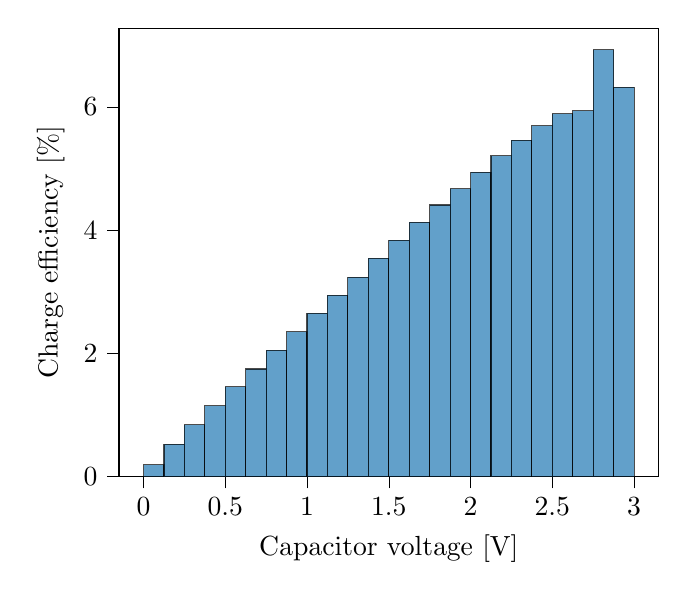
\begin{tikzpicture}

\definecolor{darkgray176}{RGB}{176,176,176}
\definecolor{steelblue31119180}{RGB}{31,119,180}

\begin{axis}[
tick align=outside,
tick pos=left,
x grid style={darkgray176},
xlabel={Capacitor voltage [V]},
xmin=-0.15, xmax=3.15,
xtick style={color=black},
y grid style={darkgray176},
ylabel={Charge efficiency [\%]},
ymin=0, ymax=7.27860203606282,
ytick style={color=black}
]
\draw[draw=black,fill=steelblue31119180,opacity=0.7] (axis cs:0,0) rectangle (axis cs:0.125,0.190539308106177);
\draw[draw=black,fill=steelblue31119180,opacity=0.7] (axis cs:0.125,0) rectangle (axis cs:0.25,0.5224581833378);
\draw[draw=black,fill=steelblue31119180,opacity=0.7] (axis cs:0.25,0) rectangle (axis cs:0.375,0.840459998601059);
\draw[draw=black,fill=steelblue31119180,opacity=0.7] (axis cs:0.375,0) rectangle (axis cs:0.5,1.1482255420802);
\draw[draw=black,fill=steelblue31119180,opacity=0.7] (axis cs:0.5,0) rectangle (axis cs:0.625,1.45566965071456);
\draw[draw=black,fill=steelblue31119180,opacity=0.7] (axis cs:0.625,0) rectangle (axis cs:0.75,1.74581675388377);
\draw[draw=black,fill=steelblue31119180,opacity=0.7] (axis cs:0.75,0) rectangle (axis cs:0.875,2.05158004481653);
\draw[draw=black,fill=steelblue31119180,opacity=0.7] (axis cs:0.875,0) rectangle (axis cs:1,2.35445880106922);
\draw[draw=black,fill=steelblue31119180,opacity=0.7] (axis cs:1,0) rectangle (axis cs:1.125,2.65015381080957);
\draw[draw=black,fill=steelblue31119180,opacity=0.7] (axis cs:1.125,0) rectangle (axis cs:1.25,2.93998251900657);
\draw[draw=black,fill=steelblue31119180,opacity=0.7] (axis cs:1.25,0) rectangle (axis cs:1.375,3.23486374921233);
\draw[draw=black,fill=steelblue31119180,opacity=0.7] (axis cs:1.375,0) rectangle (axis cs:1.5,3.54318558568533);
\draw[draw=black,fill=steelblue31119180,opacity=0.7] (axis cs:1.5,0) rectangle (axis cs:1.625,3.83884755783891);
\draw[draw=black,fill=steelblue31119180,opacity=0.7] (axis cs:1.625,0) rectangle (axis cs:1.75,4.12467720635155);
\draw[draw=black,fill=steelblue31119180,opacity=0.7] (axis cs:1.75,0) rectangle (axis cs:1.875,4.40773631237346);
\draw[draw=black,fill=steelblue31119180,opacity=0.7] (axis cs:1.875,0) rectangle (axis cs:2,4.67336702638427);
\draw[draw=black,fill=steelblue31119180,opacity=0.7] (axis cs:2,0) rectangle (axis cs:2.125,4.94093814722085);
\draw[draw=black,fill=steelblue31119180,opacity=0.7] (axis cs:2.125,0) rectangle (axis cs:2.25,5.20552331493076);
\draw[draw=black,fill=steelblue31119180,opacity=0.7] (axis cs:2.25,0) rectangle (axis cs:2.375,5.45584743400769);
\draw[draw=black,fill=steelblue31119180,opacity=0.7] (axis cs:2.375,0) rectangle (axis cs:2.5,5.6970791701015);
\draw[draw=black,fill=steelblue31119180,opacity=0.7] (axis cs:2.5,0) rectangle (axis cs:2.625,5.89212730607576);
\draw[draw=black,fill=steelblue31119180,opacity=0.7] (axis cs:2.625,0) rectangle (axis cs:2.75,5.94156609213158);
\draw[draw=black,fill=steelblue31119180,opacity=0.7] (axis cs:2.75,0) rectangle (axis cs:2.875,6.93200193910745);
\draw[draw=black,fill=steelblue31119180,opacity=0.7] (axis cs:2.875,0) rectangle (axis cs:3,6.32324320409129);
\end{axis}

\end{tikzpicture}
